\tikzstyle{box-nb} = [rectangle, minimum width=1.3cm, minimum height=0.3cm, text centered]
\tikzstyle{box} = [rectangle, minimum width=2.2cm, minimum height=0.8cm, text centered, draw=black]
\tikzstyle{arrow} = [thick,->,>=stealth]

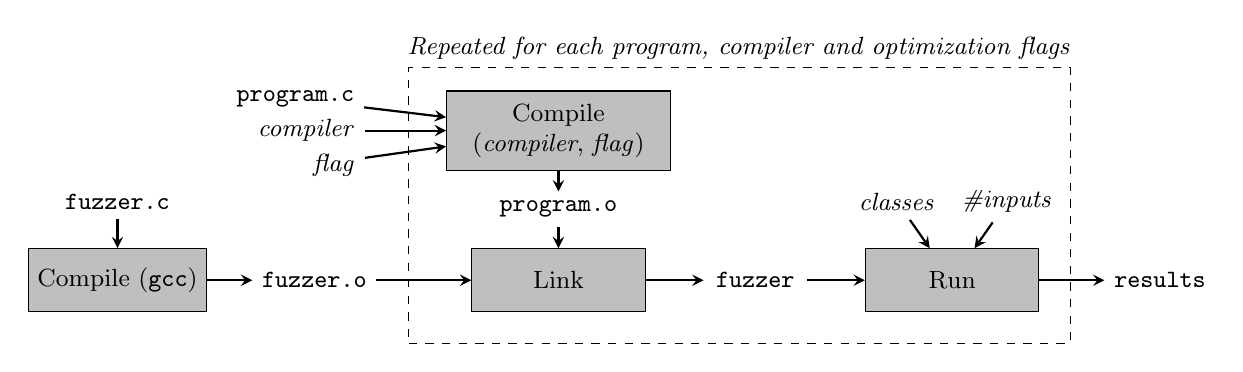
\begin{tikzpicture}
  \node (comp_prog) [box, fill=lightgray] {\small \begin{tabular}{c} Compile \\ (\textit{compiler}, \textit{flag}) \end{tabular} };
  \node (programo) [box-nb, below of=comp_prog] {\small \texttt{program.o}};
  \node (link) [box, fill=lightgray, below of=programo, yshift=0.1cm] {\small Link};
  \node (fuzzero) [box-nb, left of=link, xshift=-2.1cm] {\small \texttt{fuzzer.o}};
  \node (comp_fuzz) [box, fill=lightgray, left of=fuzzero, xshift=-1.5cm] {\small Compile (\texttt{gcc})};
  \node (fuzzerc) [box-nb, above of=comp_fuzz] {\small \texttt{fuzzer.c}};
  \node (fuzzer) [box-nb, right of=link, xshift=1.5cm] {\small \texttt{fuzzer}};
  \node (run) [box, fill=lightgray, right of=fuzzer, xshift=1.5cm] {\small Run};
  \node (classes) [box-nb, above of=run, xshift=-0.7cm] {\small \textit{classes}};
  \node (inputs) [box-nb, above of=run, xshift=0.7cm] {\small \textit{\#inputs}};
  \node (results) [box-nb, right of=run, xshift=1.64cm] {\small \texttt{results}};
  \node (programc) [box-nb, left of=comp_prog, yshift=0.4cm, xshift=-2.34cm] {\small \texttt{program.c}};
  \node (compiler) [box-nb, left of=comp_prog, xshift=-2.2cm] {\small \textit{compiler}};
  \node (flag) [box-nb, left of=comp_prog, yshift=-0.4cm, xshift=-2.13cm, yshift=-0.04cm] {\small \textit{\quad\ \ flag}};
  \node (repeat) [rectangle, draw=black, dashed, minimum height=3.5cm, minimum width=8.4cm, yshift=-0.95cm, xshift=2.3cm] {};
  \node (repeat) [box-nb, above of=repeat, yshift=1cm] {\small \textit{Repeated for each program, compiler and optimization flags}};
  
  \draw [arrow] (fuzzerc) -- (comp_fuzz);
  \draw [arrow] (comp_fuzz) -- (fuzzero);
  \draw [arrow] (comp_prog) -- (programo);
  \draw [arrow] (programo) -- (link);
  \draw [arrow] (fuzzero) -- (link);
  \draw [arrow] (link) -- (fuzzer);
  \draw [arrow] (fuzzer) -- (run);
  \draw [arrow] (run) -- (results);
  \draw [arrow] (programc) -- (comp_prog);
  \draw [arrow] (compiler) -- (comp_prog);
  \draw [arrow] (flag) -- (comp_prog);
  \draw [arrow] (classes) -- (run);
  \draw [arrow] (inputs) -- (run);
  
  \iffalse
  \node (Lexing) [box, fill=lightgray, right of=Source Code, xshift=2.5cm] {\small Lexing};
  \node (Parsing) [box, fill=lightgray, right of=Lexing, xshift=2.5cm] {\small Parsing};
  \node (AST) [box, right of = Parsing, xshift=2.5cm] {\small AST};
  \node (Semantic Analysis) [box, fill=lightgray, right of=AST, xshift=2.5cm] {\small Semantic Analysis};
  \node (Intermediate Representation) [box, below of=Semantic Analysis, yshift=-1.2cm, xshift=0cm] {\small IR};
  \node (Analysis) [box, fill=lightgray, left of=Intermediate Representation, xshift=-2.5cm] {\small Analysis};
  \node (Transformation) [box, fill=lightgray, left of=Analysis, xshift=-2.5cm] {\small Transformation};
  \node (Code Generation) [box, fill=lightgray, left of=Transformation, xshift=-2.5cm] {\small Code Generation};
  \node (Executable) [box, left of=Code Generation, xshift=-2.5cm] {\small Executable};
  \draw [arrow] (Source Code) -- (Lexing);
  \draw [arrow] (Lexing) -- (Parsing);
  \draw [arrow] (Parsing) -- node [fill=white, text=darkgray, yshift=0.7cm] {\small Syntactically Sound} (AST);
  \draw [arrow] (AST) -- (Semantic Analysis);
  \draw [arrow] (Semantic Analysis) -- node [fill=white, text=darkgray] {\small Semantically Sound} (Intermediate Representation);
  \draw [arrow] (Intermediate Representation) -- (Analysis);
  \draw [arrow] (Analysis) -- (Transformation);
  \draw [arrow, dashed] (Transformation) to [bend left=25] (Intermediate Representation);
  \draw [arrow] (Transformation) -- node [fill=white, text=red, yshift=0.7cm] {\small Optimized} (Code Generation);
  \draw [arrow] (Code Generation) -- (Executable);
\fi
\end{tikzpicture}